% !TEX TS-program = pdflatex
% !TEX encoding = UTF-8 Unicode

% This is a simple template for a LaTeX document using the "article" class.
% See "book", "report", "letter" for other types of document.

%tells you if you use obsolote packages
%\RequirePackage[l2tabu,orthodox]{nag}

\documentclass[]{article}

\usepackage[utf8]{inputenc} % set input encoding (not needed with XeLaTeX)

%%% PAGE DIMENSIONS
\usepackage{geometry} % to change the page dimensions
\geometry{a4paper} % or letterpaper (US) or a5paper or....
% \geometry{margin=2in} % for example, change the margins to 2 inches all round
% \geometry{landscape} % set up the page for landscape
%   read geometry.pdf for detailed page layout information

\usepackage{graphicx} % support the \includegraphics command and options

% \usepackage[parfill]{parskip} % Activate to begin paragraphs with an empty line rather than an indent

%%% PACKAGES
\usepackage{booktabs} % for much better looking tables
\usepackage{array} % for better arrays (eg matrices) in maths
\usepackage{paralist} % very flexible & customisable lists (eg. enumerate/itemize, etc.)
\usepackage{verbatim} % adds environment for commenting out blocks of text & for better verbatim
\usepackage{subfig} % make it possible to include more than one captioned figure/table in a single float
\usepackage{microtype} %makes awesome kerning and punctuation come half way out the edge of the text
\usepackage{listings} %for code listings
\usepackage{color} %for colored syntax highligting

%%% Code listing
\definecolor{mygreen}{rgb}{0,0.6,0}
\definecolor{mygray}{rgb}{0.5,0.5,0.5}
\definecolor{mymauve}{rgb}{0.58,0,0.82}
\lstset{breaklines=true,
basicstyle=\footnotesize\ttfamily,
commentstyle=\color{mygreen},
keywordstyle=\color{blue},
numberstyle=\tiny\color{mygray},
tabsize=2,
language=c
}

% to include a file as a listing: \lstinputlisting{intio.c}
% inline listing: \begin{lstlisting}[frame=single]

%%% HEADERS & FOOTERS
\usepackage{fancyhdr} % This should be set AFTER setting up the page geometry
\pagestyle{fancy} % options: empty , plain , fancy
\renewcommand{\headrulewidth}{0pt} % customise the layout...
\lhead{}\chead{}\rhead{}
\lfoot{}\cfoot{\thepage}\rfoot{}

%%% ToC (table of contents) APPEARANCE
\usepackage[nottoc,notlof,notlot]{tocbibind} % Put the bibliography in the ToC
\usepackage[titles,subfigure]{tocloft} % Alter the style of the Table of Contents
%\renewcommand{\cftsecfont}{\rmfamily\mdseries\upshape}
%\renewcommand{\cftsecpagefont}{\rmfamily\mdseries\upshape} % No bold!
\usepackage{hyperref} % use hyperlinked ToC
\hypersetup{colorlinks=true, linkcolor=black}

%%%-------------------------------------------------------------------


\title{Title Here}
\author{Oskar Weigl - ow610\\ and \\ Ryan Savitski - rs510}
%\date{} % Activate to display a given date or no date (if empty),
         % otherwise the current date is printed 

\begin{document}
\maketitle

%\renewcommand{\abstractname}{Summary}
\begin{abstract}
	Write the abstract here
\end{abstract}

\tableofcontents
\clearpage


\section{Notch Filter} % (fold)
\label{sec:notch_filter}

\begin{figure}[htbp]
	\begin{center}
		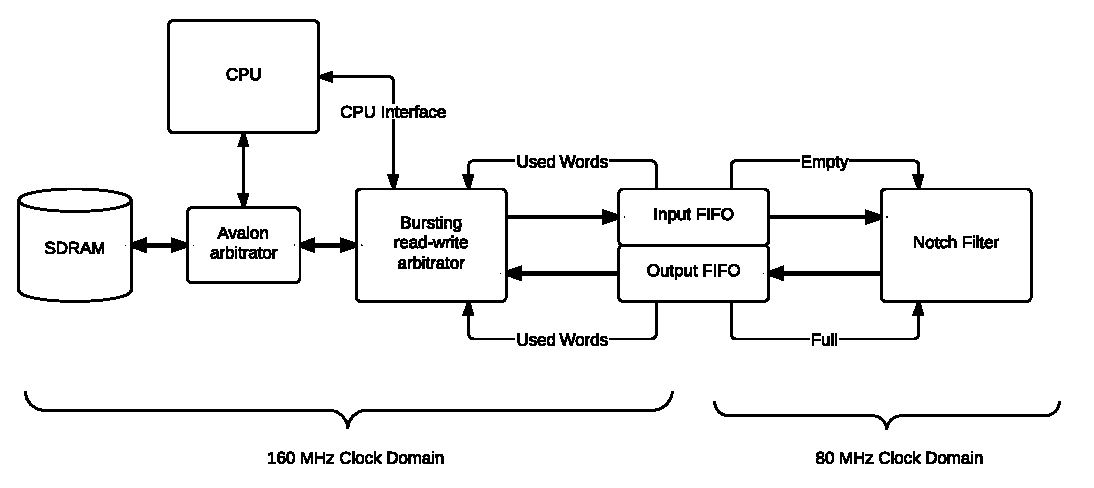
\includegraphics[width = \textwidth]{DSDNotch.pdf}
	\end{center}
	\caption{Block diagram of the Notch Filter hardware. FIFO buffers are used to allow efficient interleaved reads and writes to SDRAM. The buffers also serve as Clock Domain Crossing interfaces.}
	\label{fig:DSDNotch}
\end{figure}


The Notch Filter module is a memory mapped hardware accelerator for the purpose of filtering a 16 bit signed input. It is a 2nd order notch filter tuned to to remove any spectral components at 1 kHz.
The module is capable of Direct Memory Access, and includes optimisations for efficient access to the SDRAM, and uses a buffering, and Clock Domain Crossing strategy, to maximise performance.


\subsection{Filter Design} % (fold)
\label{sub:filter_design}

\begin{figure}[htbp]
	\begin{center}
		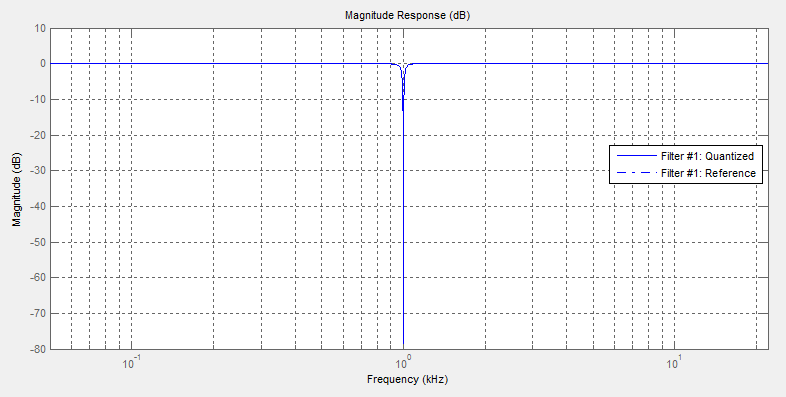
\includegraphics[width = \textwidth]{matlabmagnitudelog.PNG}
	\end{center}
	\caption{Magnitude response of both the full (double) precision and the quantised filter. The gain is negative infinity dB at 1 kHz.}
	\label{fig:matlabmagnitudelog}
\end{figure}

The chosen filter type is a 2nd order notch filter. This filter order is the minimum required to generate the complex pole and zero pairs required to implement a notch filter. In fact, no higher order is needed, as the noise is a pure sinusoid, so the width of the stop-band can be very small, and as such, there are no additional zeroes required.

The filter is designed by simply placing a complex zero pair on the unit circle corresponding to the 1 KHz null we wish to create. To cancel the effect of this zero for other frequencies, we place a pole very close to it on the inside of the unit circle. The bandwidth of the filter is tuned by moving the complex pole radially.

In our case, we elect to place the pole such that the bandwidth of rejection is about 25Hz. This is was chosen as a good trade-off for several reasons. Firstly, placing the pole at this location makes the filter robust to coefficient quantisation, as discussed in Section~\ref{sub:quantization}.
More importantly, this bandwidth is narrow enough to not affect the music, but wide enough to quickly suppress the overlaid sinusoid at the beginning of the sample.
The magnitude of the resulting filter can been seen in Figure~\ref{fig:matlabmagnitudelog}.

% subsection filter_design (end)

\subsection{Filter Topology} % (fold)
\label{sub:filter_topology}

Several different types of filter topologies were considered. It is clear that as a 2nd order 

The effects of quantization depends entirely on the chosen filter topology. 

% subsection filter_topology (end)

\subsection{Quantization} % (fold)
\label{sub:quantization}



% subsection quantization (end)



\subsection{Architecture} % (fold)
\label{sub:architecture}

Assesment of speed (critical path) of different filter stuctures
Describe diagram 1, (SDRAM slow, but good for sequential, interleaving)

% subsection architecture (end)




\begin{figure}[htbp]
	\begin{center}
		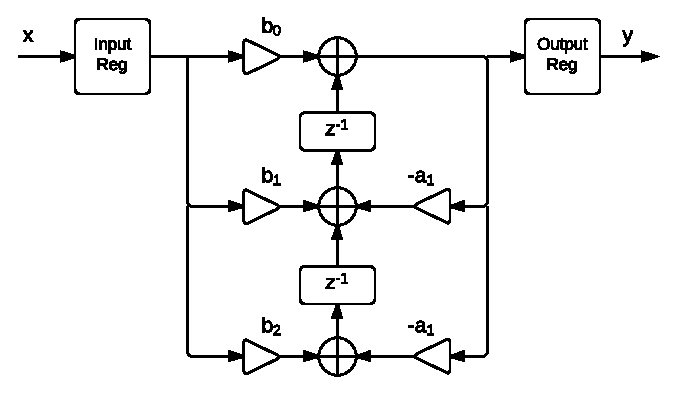
\includegraphics[width = 0.8\textwidth]{DirectFormIITransposed.pdf}
	\end{center}
	\caption{Second order Direct Form II Transposed filter architecture}
	\label{fig:df2t}
\end{figure}

\begin{figure}[htbp]
	\begin{center}
		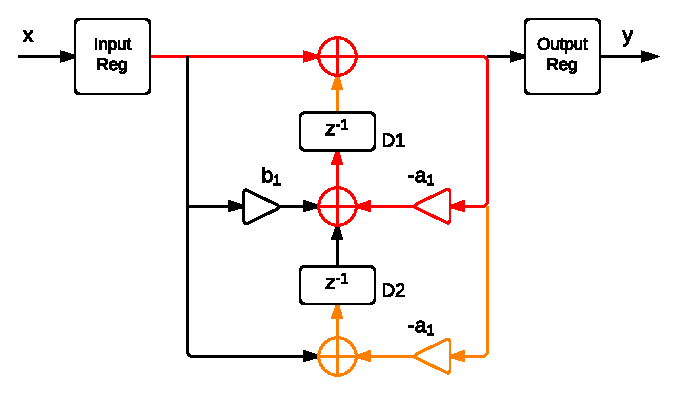
\includegraphics[width = 0.8\textwidth]{DirectFormIITransposedCritpath.pdf}
	\end{center}
	\caption{Annotated version of Figure~\ref{fig:df2t}, showing the main critical paths in the filter core. Shown in red is the path from the input register to the delay register D1. Shown in orange are the alternative paths that have almost as little slack as the red path.}
	\label{fig:df2tCritpath}
\end{figure}

\pagebreak




% section notch_filter (end)

\end{document}
